\newpage
\chapter{Vector Bundles}\label{ch2}
Let $\B$ denote a fixed topological space, which will be called the
base space.
\begin{definition}\label{def:2-1}
	A real vector bundle $\xi$ over $\B$ consists of the 
	following:
	\begin{enumerate}[label=\arabic*),leftmargin=2\parindent ]
		\item a topological space $E=
		E(\xi)$ called the \textit{total space},
		\item  a (continuous) map $\pi\mathpunct{:} E \to \B$ called the \textit{projection map}, and
		\item  for each $b\in \B$ the structure of a vector space\footnote{To be more precise this vector space structure could be specified by giving
			the subset of $\R\times\R\times E\times E\times E$ consisting of all $5$-tuples $(t_1,t_2,e_1,e_2,e_3)$ with \[\pi(e_1)=\pi(e_2) = \pi(e_3)\quad\text{and}\quad e_3 = t_1e_1 + t_2e_2.\]} over the real 
		numbers in the set $\pi\inv(b)$.
	\end{enumerate}
\end{definition}

These must satisfy the following restriction:

Condition of \textit{local triviality}. For each point $b$ of $\B$ there should
exist a neighborhood $U \subset \B$, an integer $n \geq 0$, and a homeomorphism
\[h\mathpunct{:}U\times \R^n\longrightarrow\pi\inv(U),\]
so that, for each $b\in U$, the correspondence $x \to h(b, x)$ defines an isomorphism between the vector space $\R^n$ and the vector space $\pi\inv(b)$.

Such a pair $(U, h)$ will be called a \textit{local coordinate system for $\xi$
about $b$}. If it is possible to choose $U$ equal to the entire base space,
then $\xi$ will be called a \textit{trivial bundle}.

The vector space $\pi\inv(b)$ is called the \textit{fiber over} $b$. It may be 
denoted by $F_b$ or
$F_b(\xi)$. Note that $F_b$ is never vacuous, although it may
consist of a single point. The dimension $n$ of $F_b$ is allowed to be a (locally constant) function of $b$; but in most cases of interest this 
function is constant. One then speaks of an $n$\textit{-plane bundle}, or briefly an $\R^n$-\textit{bundle}.

The concept of a \textit{smooth vector bundle} can be defined similarly. One
requires that $\B$ and $E$ be smooth manifolds, that $\pi$ be a smooth map,
and that, for each $b\in \B$ there exist a local coordinate system $(U, h)$
with $b \in U$ such that $h$ is a diffeomorphism.

\begin{remark}
	An $\R^n$-bundle is a very special example of a fiber bundle.
	(See \cite[p. 9]{18}.) In Steenrod's terminology an $\R^n$-bundle is a
	fiber bundle with fiber $\R^n$ and with the full linear group $\mathbf{GL}(n,\R)$ in $n$
	variables as structural group.
\end{remark}

Now consider two vector bundles $\xi$ and $\eta$ over the same base space
$\B$.

\begin{definition}\label{def:2-2}
	$\xi$ is \textit{isomorphic} to $\eta$, written $\xi \cong \eta$, if there exists
	a homeomorphism $f\mathpunct{:}E(\xi)\to E(\eta)$ between the total spaces which maps each vector space $F_b(\xi)$ isomorphically onto the corresponding vector space $F_b(\eta)$.
	
\end{definition}

\begin{example}
	The trivial bundle with total space $\B \times \R^n$, with 
	projection map $\pi(h, x) =
	b$, and with the vector space structures in the fibers
	defined by
	\[t_1(b,x_1) +
	t_2(b,x_2) =
	(b,t_1x_1 +
	t_2x_2) ,\]
	will be denoted by $\mathcal{E}^n_\B$. Note that a second $\R^n$-bundle over $\B$ is trivial
	if and only if it is isomorphic to $\mathcal{E}^n_\B$.
\end{example}

\begin{example}
	The \textit{tangent bundle} $\tau_M$ of a smooth manifold $M$. The
	total space of $\tau_M$ is the manifold $DM$ consisting of all pairs $(x,v)$ with
	$x \in M$ and $v$ tangent to $M$ at $x$. The projection map $\pi\mathpunct{:}DM \to M$
	is defined by $\pi(x, v) =
	x$; and the vector space structure in $\pi\inv(x)$ is
	defined by
	\[t_1(x,v_1) +
	t_2(x,v_2) =
	(x,t_1v_1 + t_2v_2). \]
	
	The local triviality condition is not difficult to verify. Note that $\tau_M$ is
	an example of a smooth vector bundle.
\end{example}

If $\tau_M$ is a trivial bundle, then the manifold $M$ is called parallelizable.
For example suppose that $M$ is an open subset of $\R^n$. Then $DM$ is
equal to $M \times \R^n$, and $M$ is clearly parallelizable.

The unit $2$-sphere $\Sphere{2}\subset \R^3$ provides an example of a manifold which
is not parallelizable. (Compare \cref{prob-2-B}.) In fact we will see in \cref{ch-9}
that a parallelizable manifold must have Euler characteristic zero, whereas
the $2$-sphere has Euler characteristic $+2$. (See \cref{cor-9-3} and \cref{thm-11-6}.)

\begin{example}\label{ex-2-3}
	The normal bundle $\nu$ of a smooth manifold $M \subset \R^n$ is
	obtained as follows. The total space
	$E \subset M \times \R^n$
	is the set of all pairs $(x, v)$ such that $v$ is orthogonal to the tangent
	space $DM$ . The projection map $\pi\mathpunct{:} E \to M$ and the vector space 
	structure in $\pi\inv(x)$ are defined, as in \cref{ex-1,ex-2}, by the formulas $\pi(x, v) =
	x$, and $t_1(x, v_1) +
	t_2(x, v_2) =
	(x, t_1v_1 +
	t_2v_2)$. The proof that $\nu$ satisfies
	the local triviality condition will be deferred until \S 3.4.
\end{example}
\begin{example}\label{ex-2-4}
	 The \textit{real projective space} $\rp{n}$ can be defined\footnote{Alternatively $\rp{n}$ can be defined as the set of lines through the origin in
	$\R^{n+1}$.
	(Compare \cref{prob-1-b}.) This amounts to the same thing since every
	such line cuts $\Sphere{n}$ in two antipodal points.} as the
set of all unordered pairs $\{x, -x\}$ where $x$ ranges over the unit sphere
$\Sphere{n} \subset\R^{n+1}$; and is topologized as a quotient space of $\Sphere{n}$.

Let $E(\gamma^1_n)$ be the subset of $\rp{n}\times \R^{n+1}$ consisting of all pairs
$(\{\pm x\}, v)$ such that the vector $v$ is a multiple of $x$. Define $\pi\mathpunct{:} E(\gamma^1_n)\to \rp{n}$
	by $\pi(\{\pm x\} , v) =
		\{\pm x\}$. Thus each fiber $\pi\inv(\{\pm x\})$ can be identified with
		the line through $x$ and $-x$ in $\R^{n+1}$. Each such line is to be given its
		usual vector space structure. The resulting vector bundle $\gamma^1_n$ will be
		called the \textit{canonical line bundle} over $\rp{n}$.
		
		\begin{proof}
			[\textsc{Proof that $\gamma^1_n$ is locally trivial.}] Let $U \subset \Sphere{n}$ be any open set which
			is small enough so as to contain no pair of antipodal points, and let $U_1$
			denote the image of $U$ in $\rp{n}$. Then a homeomorphism
			\[h\mathpunct{:}U_1\times \R^n\longrightarrow\pi\inv(U_1),\]
			is defined by the requirement that $h(\{\pm x\},t)=(\{\pm x\},tx)$ for each $(x, t)\in U \times \R$. Evidently $(U_1,h)$ is a local coordinate system;
			hence $\gamma^1_n$ is locally trivial.
		\end{proof}
\end{example}

\begin{theorem}\label{thm-2-1}
	The bundle $\gamma^1_n$ over $\rp{n}$ is not trivial, for
	$n \geq 1$.
\end{theorem}
\begin{definition}\label{def:2-3}
	A \textit{cross-section} of a vector bundle $\xi$ with base space
	$\B$ is a continuous function $s\mathpunct{:}\B\to E(\xi)$ which takes each $b \in \B$ into the corresponding fiber $F_b (\xi)$. Such a
	cross-section is \textit{nowhere zero} if $s(b)$ is a non-zero vector of $F_b (\xi)$ for
	each $b$. 
	
	(A cross-section of the tangent bundle of a smooth manifold $M$ is
	usually called a \textit{vector field} on $M$.)
	
\end{definition}

Evidently a trivial $\R$-bundle possesses a cross-section which is nowhere zero. We will see that the bundle $\gamma^1_n$ has no such cross-section.

Let
$s\mathpunct{:}\rp{n}\longrightarrow E(\gamma^1_n)$
be any cross-section, and consider the composition
\[\Sphere{n}\xrightarrow{\quad \ \quad}\rp{n}\xrightarrow{\quad s\quad} E(\gamma^1_n)\]
which carries each $x \in\Sphere{n}$ to some pair $\left(\{\pm x\},t(x)x\right)\in E(\gamma^1_n)$. Evidently $t(x)$ is a continuous real valued function of $x$, and $t(-x)=-t(x)$.
Since $\Sphere{n}$ is connected it follows from the intermediate value theorem
that $ t(x_0) = 0 $ for some
$x_0$. Hence $s(\{\pm x_0\})=(\{\pm x_0\},0)$. This completes
		the proof.\qed
		

It is interesting to take a closer look at the space $E(\gamma^1_n)$ for the 
special case $n = 1$. In this case each point $e =
(\{\pm x\}, v)$ of $E(\gamma^1_n)$ can be
written as
\[e =
(\{\pm(\cos \theta, \sin \theta)\}, t(\cos \theta, \sin \theta)), \]
with $0 \leq \theta \leq \pi$, $t\in \R$. This representation is unique except that the point
$(\{\pm(\cos 0, \sin 0)\}, t(\cos 0, \sin 0))$ is equal to $(\{\pm(\cos \pi, \sin \pi)\}, -t(\cos \pi, \sin \pi))$ for each $t$. In other words $E(\gamma^1_1)$ can be obtained from
	the strip $[0,\pi]\times \R$ in the $(\theta, t)$-plane by identifying the left hand 
	boundary $[0]\times \R$ with the right hand boundary $[\pi]\times \R$ under the 
	correspondence $(0,t) \mapsto (\pi,-t)$. Thus $E(\gamma^1_1)$ is an open Moebius band. (Compare
	\cref{fig2}.)
	
	This description gives an alternative proof that $\gamma^1_1$ is non-trivial.
	For the Moebius band is certainly not homeomorphic to the cylinder
	$\rp{1}\times \R$.
	
	\begin{figure}[!htb]
		\centering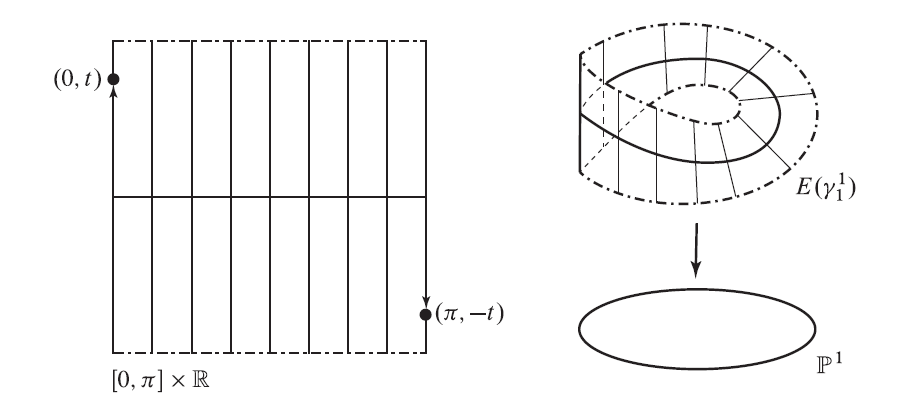
\includegraphics[scale=.5]{fig2}
		\caption{}\label{fig2}
	\end{figure}

Now consider a collection $\set{a^3}\ntuple{V_n}\base{x} \set{S_{10}}$ of cross-sections of a vector
bundle $\xi$.

\begin{definition}\label{def:2-4}
	 The cross-sections $\coord{s_n}$ are \textit{nowhere depend}
	if, for each $b \in \B$, the vectors $\coord{s_nb}$ are linearly independent.
\end{definition}
\begin{theorem}\label{thm-2-2}
	An $\R^n$-bundle $\xi$ is trivial if and only if $\xi$ admits $n$ cross-sections $\coord{s_nb}$ which are nowhere dependent.
\end{theorem}

The proof will depend on the following basic result.
\begin{lemma}\label{lem-2-3}
	Let $\xi$ and $\eta$ be vector bundles over $\B$ and let
	$f\mathpunct{:} E(\xi) \rightarrow E(\eta)$ be a continuous function which maps each vector space $F_{b}(\xi)$ isomorphically onto the corresponding vector space $F_{b}(\eta)$. Then $f$ is necessarily a homeomorphism. Hence
	$\xi$ is isomorphic to $\eta$.
\end{lemma}
\begin{proof}
	Given any point $b \in \B$, choose local coordinate systems
	$(U,g)$ for $\xi$ and $(V,h)$ for $\eta$, with $b_{0} \in U \cap V$. Then we must show
	that the composition
	\[(U \cap V) \times \mathbb{R}^{n} \xrightarrow{h^{-1} \circ f \circ g}(U \cap V) \times \mathbb{R}^{n},\]
	is a homeomorphism. Setting
	\[h\inv(f(g(b, x)))=(b, y),\]
	it is evident that $y =\ntuple{y_n}$ can be expressed in the form
	\[y_{i}=\sum_{j} f_{i j}(b) x_{j},\]
	where $[f_{i j}(b)]$ denotes a non-singular matrix of real numbers. 
	Furthermore the entries $f_{i j}(b)$ depend continuously on $b$. Let $[F_{ji}(b)]$ denote
	the inverse matrix. Evidently
	\[g^{-1} \circ f^{-1} \circ h(b, y)=(b, x), \]
	where
	\[x_{j}=\sum_{i} F_{ji}(b) y_{i},\]
	Since the numbers $F_{ji}(b)$ depend continuously on the matrix $[f_{i j}(b)]$,
	they depend continuously on $b$. Thus $g^{-1} \circ f^{-1} \circ h$ is continuous, which
	completes the proof of \cref{lem-2-3}.
\end{proof}
\begin{proof}[Proof of \cref{thm-2-2}. ]
	Let $\coord{s_n}$ be cross-sections of $\xi$ which
	are nowhere linearly dependent. Define
$f\mathpunct{:} \B \times \R^{n} \rightarrow E$ by
			\[f(b, x)=x_{1} s_{1}(b)+\cdots+x_{n} s_{n}(b).\]
 Evidently $f$ is continuous and maps each fiber of the trivial bundle $\mathcal{E}^n_\B$
 isomorphically onto the corresponding fiber of $\xi$. Hence $f$ is a bundle
 isomorphism, and $\xi$ is trivial.
 
 Conversely suppose that $\xi$ is trivial, with coordinate system $(B, h)$. Defining
 \[s_{i}(b)=h(b,(0, \dots, 0,1,0, \dots, 0)) \in F_{b}(\xi)\]
 (with the $1$ in the $i$-th place), it is evident that $\coord{s_n}$ are nowhere
 dependent cross-sections. This completes the proof.
\end{proof}

As an illustration, the tangent bundle of the circle $\Sphere{1} \subset \R^2$ admits
one nowhere zero cross-section, as illustrated in \cref{fig3}. (The indicated
arrows lead from $x\in\Sphere{1}$  to $x + v$, where $s(x) =
(x, v) =((x_1,x_2), (-x_2,x_1))$.)
Hence $\Sphere{1}$  is parallelizable. Similarly the $3$-sphere $\Sphere{3}\subset\R^4 $ admits
three nowhere dependent vector fields $s_{i}(x)=\left(x, \bar{s}_{i}(x)\right)$ where
\begin{align*}
		\bar{s}_{1}(x)&=\left(-x_{2}, x_{1},-x_{4}, x_{3}\right), \\
		\bar{s}_{2}(x)&=\left(-x_{3}, x_{4}, x_{1},-x_{2}\right), \\
		\bar{s}_{3}(x)&=\left(-x_{4},-x_{3}, x_{2}, x_{1}\right).
\end{align*}
Hence $\Sphere{3}$ is parallelizable. (These formulas come from the quaternion
multiplication in $\R^4$.
Compare \cite[\S 8.5]{18}.)
\begin{figure}[!htb]
	\centering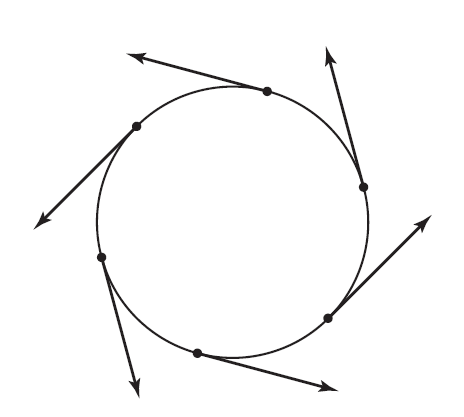
\includegraphics[scale=.6]{fig3}
	\caption{}\label{fig3}
\end{figure}


\section*{Euclidean Vector Bundles}
For many purposes it is important to study vector bundles in which
each fiber has the structure of a Euclidean vector space.

Recall that a real valued function $\mu$ on a finite dimensional vector
space $V$ is \textit{quadratic} if $\mu$ can be expressed in the form
\[\mu(v)=\sum \ell_{i}(v) \ell_{i}^{\prime}(v),\]
where each $\ell_{i}$ and each $\ell_{i}^{\prime}$ is linear. Each quadratic function determines
a symmetric and bilinear pairing $v, w \mapsto v \bdotp
w$ from $V\times V$ to $\R$, where
\[v \bdotp w=\frac{1}{2}(\mu(v+w)-\mu(v)-\mu(w)).\]
Note that $v \bdotp
v =
\mu(v)$. The quadratic function $\mu$ is called \textit{positive
definite} if $\mu(v) > 0$ for $v\neq 0$.

\begin{definition}\label{def:2-5}
	A \textit{Euclidean vector space} is a real vector space $V$
	together with a positive definite quadratic function
	\[\mu\mathpunct{:}V\longrightarrow \R. \]
	The real number $v \bdotp w$ will be called the \textit{inner product} of the vectors $v$
	and $w$. The number $v\bdotp v =\mu(v)$ may also be denoted by $|v|^2$.
\end{definition}


\begin{definition}\label{def:2-6}
	A \textit{Euclidean vector bundle} is a real vector bundle $\mu$
	together with a continuous function
\[\mu\mathpunct{:}E(\xi) \longrightarrow \R,\]
	such that the restriction of $\mu$ to each fiber of $\xi$ is positive definite and
	quadratic. The function $\mu$ itself will be called a \textit{Euclidean metric} on
	the vector bundle $\xi$.
	
	In the case of the tangent bundle $\tau_M$ of a smooth manifold, a 
	Euclidean metric
	\[\mu\mathpunct{:}DM \longrightarrow \R,\]
	is called a \textit{Riemannian metric}, and $M$ together with $\mu$ is called a 
	\textit{Riemannian manifold}. (In practice one usually requires that $\mu$ be a smooth
	function. The notation  $\mu=
	ds^2$ is often used for a Riemannian metric.)
\end{definition}
\begin{note}
	In Steenrod's terminology a Euclidean metric on $\xi$ gives rise
	to a reduction of the structural group of $\xi$ from the full linear group to
	the orthogonal group. Compare \cite[\S 12.9]{18}.
\end{note}

\begin{example}\label{ex-0-0}
	The trivial bundle $\mathcal{E}^n_\B$ can be given the Euclidean metric
	\[\mu(b, x)=x_{1}^{2}+\cdots+x_{n}^{2}.\]
	Since the tangent bundle of $\R^n$ is trivial it follows that the smooth 
	manifold $\R^n$ possesses a standard Riemannian metric. For any smooth 
	manifold $M \subset \R^n$ the composition
\[DM\subset D\R^n\xrightarrow{\quad\mu\quad} \R, \]
now makes $M$ into a Riemannian manifold.
\end{example}
A priori there appear to be two different concepts of triviality for
Euclidean vector bundles; however the next lemma shows that these coincide.

\begin{lemma}\label{lem-2-4}
	Let $\xi$ be a trivial vector bundle of dimension $n$
	over $\B$, and let $\mu$ be any Euclidean metric on $\xi$. Then there
	exist $n$ cross-sections $\coord{s_n}$ of $\xi$ which are normal and
	orthogonal in the sense that
	$s_i(b)\bdotp s_j(b)=\delta_{ij}$
	for each $b\in\B$.
\end{lemma}

Thus $\xi$ is trivial also as a Euclidean vector bundle. (Compare
\cref{prob-2-E} below.)
\begin{proof}
	Let $\coord{{s'}_n}$ be any $n$ cross-sections which are nowhere
	linearly dependent. Applying the Gram-Schmidt\footnote{See any text book on linear algebra.} process to $\coord{{s'}_nb}$
	we obtain a normal orthogonal basis $\coord{s_nb}$ for $F_b(\xi)$. Since
	the resulting functions $\coord{s_n}$ are clearly continuous, this completes
	the proof, 
\end{proof}
\section*{Problems}
Here are six problems for the reader.
\begin{problem}\label{prob-2-A}
	Show that the unit sphere $\Sphere{n}$ admits a vector field
	which is nowhere zero, providing that $n$ is odd. Show that the normal
	bundle of $\Sphere{n}\subset\R^{n+1}$ is trivial for all $n$.
\end{problem}
\begin{problem}\label{prob-2-B}
	If $\Sphere{n}$ admits a vector field which is nowhere zero,
	show that the identity map of $\Sphere{n}$ is homotopic to the antipodal map. For
	$n$ even show that the antipodal map of $\Sphere{n}$ is homotopic to the reflection
	\[r\ntuple{x_{n+1}}=\left(-x_{1}, x_{2}, \ldots, x_{n+1}\right);\]
	and therefore has degree $-
	1$. (Compare \cite[p. 304]{2}.)
	Combining these facts, show that $\Sphere{n}$ is not parallelizable for $n$ even,
	$n \geq 2$.
\end{problem}
\begin{problem}[Existence theorem for Euclidean metrics.]\label{prob-2-C}
 Using a 
partition of unity, show that any vector bundle over a paracompact base
space can be given a Euclidean metric. (See \S \ref{sec5.8}; or see \cite[pp. 156
and 171]{41}.)
\end{problem}
\begin{problem}\label{prob-2-D}
	The Alexandroff line $L$ (sometimes called the ``long
	line") is smooth, connected, $1$-dimensional manifold which is not 
	paracompact. (Reference: \cite{42}.) Show that $L$ cannot be given a Riemannian metric.
\end{problem}
\begin{problem}[Isometry theorem.]\label{prob-2-E}
 Let $\mu$ and $\mu'$ be two different
Euclidean metrics on the same vector bundle $\xi$. Prove that there exists
a homeomorphism $f\mathpunct{:} E(\xi)\to
E(\xi)$ which carries each fiber isomorphically
onto itself, so that the composition  $\mu\circ f\mathpunct{:} E(\xi)\to
\R$ is equal to $\mu'$. [Hint:
Use the fact that every positive definite matrix $A$ can be expressed
uniquely as the square of a positive definite matrix $\sqrt{A}$. The power
series expansion
\[\sqrt{(t\mathrm{I}+X)}=\sqrt{t}\left(\mathrm{I}+\frac{1}{2t}X-\frac{1}{8t^2}X^2+-\dots\right), \]
is valid providing that the characteristic roots of $t\mathrm{I}+X = A$ lie between
$0$ and $2t$. This shows that the function $A\mapsto \sqrt{A}$ is smooth.]
\end{problem}

\begin{problem}\label{prob-2-F}
	As in \cref{prob-1-C}, let $F$ denote the algebra of smooth
	real valued functions on $M$. For each $x\in M$ let $I^{r+1}_X$ be the ideal consisting of all functions in $F$ whose derivatives of order $\leq r$ vanish at $x$.
	An element of the quotient algebra $F/I^{r+1}_X$ is called an \textit{$r$-jet} of a real
	valued function at $x$. (Compare \cite{43}.) Construct a locally
	trivial ``bundle of algebras" $\mathcal{A}_M^{(r)}$ over $M$ with typical fiber $F/I^{r+1}_X$.
\end{problem}
